\subsubsection{UC\theuccount-GP - Aggiunta nuovo utente}
		\begin{figure}[H]
			\centering
				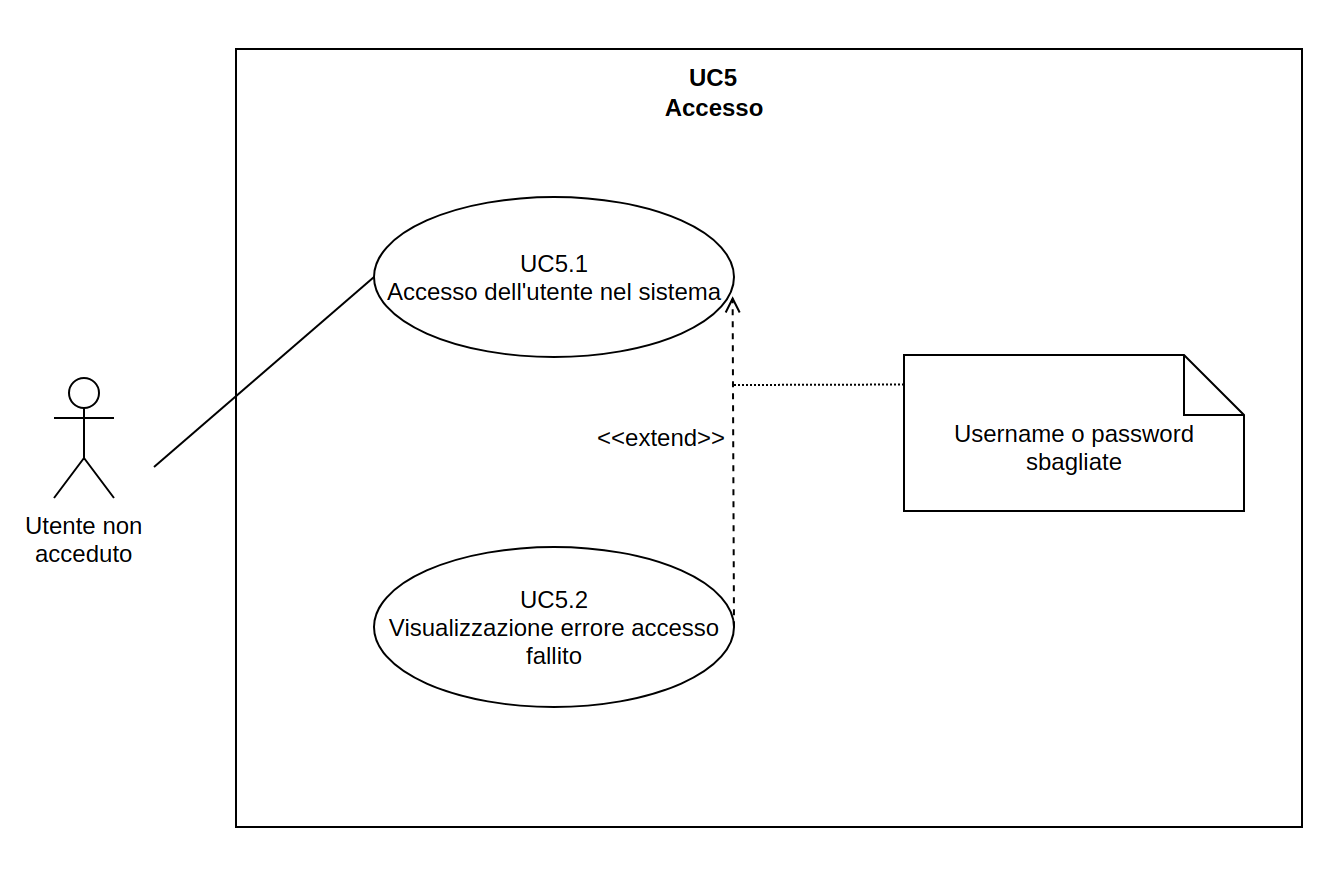
\includegraphics[width=\columnwidth]{img/UC5.png}\\
			\caption{UC\theuccount-GP - Aggiunta nuovo utente}
		\end{figure}
	\begin{itemize}
		\item \textbf{Codice}: UC\theuccount-GP.
		\item \textbf{Titolo}: aggiunta nuovo utente.
		\item \textbf{Attori primari}: utente acceduto.
		\item \textbf{Descrizione}: l'utente aggiunge un nuovo utente nel sistema.
		\item \textbf{Precondizione}: un nuovo utente deve essere aggiunto nel sistema.
		\item \textbf{Postcondizione}: un utente viene aggiunto al sistema.
		\item \textbf{Scenario Principale}:
		\begin{enumerate}
			\item Utente acceduto procede all'aggiunta di un nuovo utente.
		\end{enumerate}
	\end{itemize}

	\paragraph{UC\theuccount.1-GP - Utente aggiunto con successo}
		\begin{figure}[H]
			\centering
			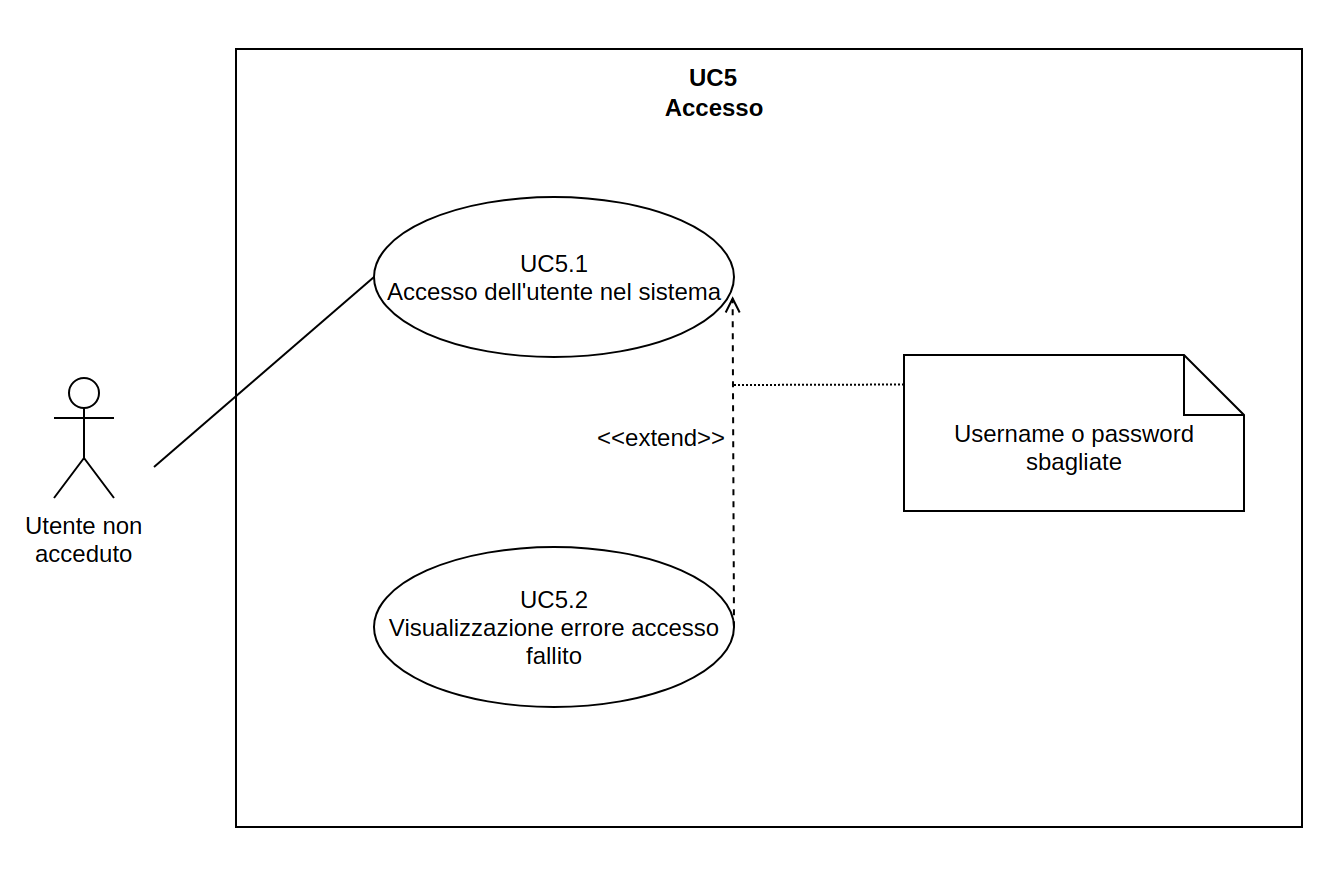
\includegraphics[width=\columnwidth]{img/UC5.png}\\
			\caption{UC\theuccount.1-GP - Utente aggiunto con successo}
		\end{figure}
		\begin{itemize}
			\item \textbf{Codice}: UC\theuccount.1-GP.
			\item \textbf{Titolo}: utente aggiunto con successo.
			\item \textbf{Attori primari}: utente acceduto.
			\item \textbf{Descrizione}: un nuovo utente viene inserito con successo nel sistema.
			\item \textbf{Precondizione}: un nuovo utente deve essere aggiunto nel sistema.
			\item \textbf{Postcondizione}: un utente viene aggiunto al sistema.
			\item \textbf{Scenario Principale}:
			\begin{enumerate}
				\item Utente acceduto procede all'aggiunta di un nuovo utente.
			\end{enumerate}
			\item \textbf{Estensioni}:
			\begin{itemize}
				\item Errore utente già presente nel sistema[UC13-GP].
			\end{itemize}
		\end{itemize}

		\subparagraph{UC\theuccount.1.1-GP - Inserimento nome utente}
			\begin{figure}[H]
				\centering
				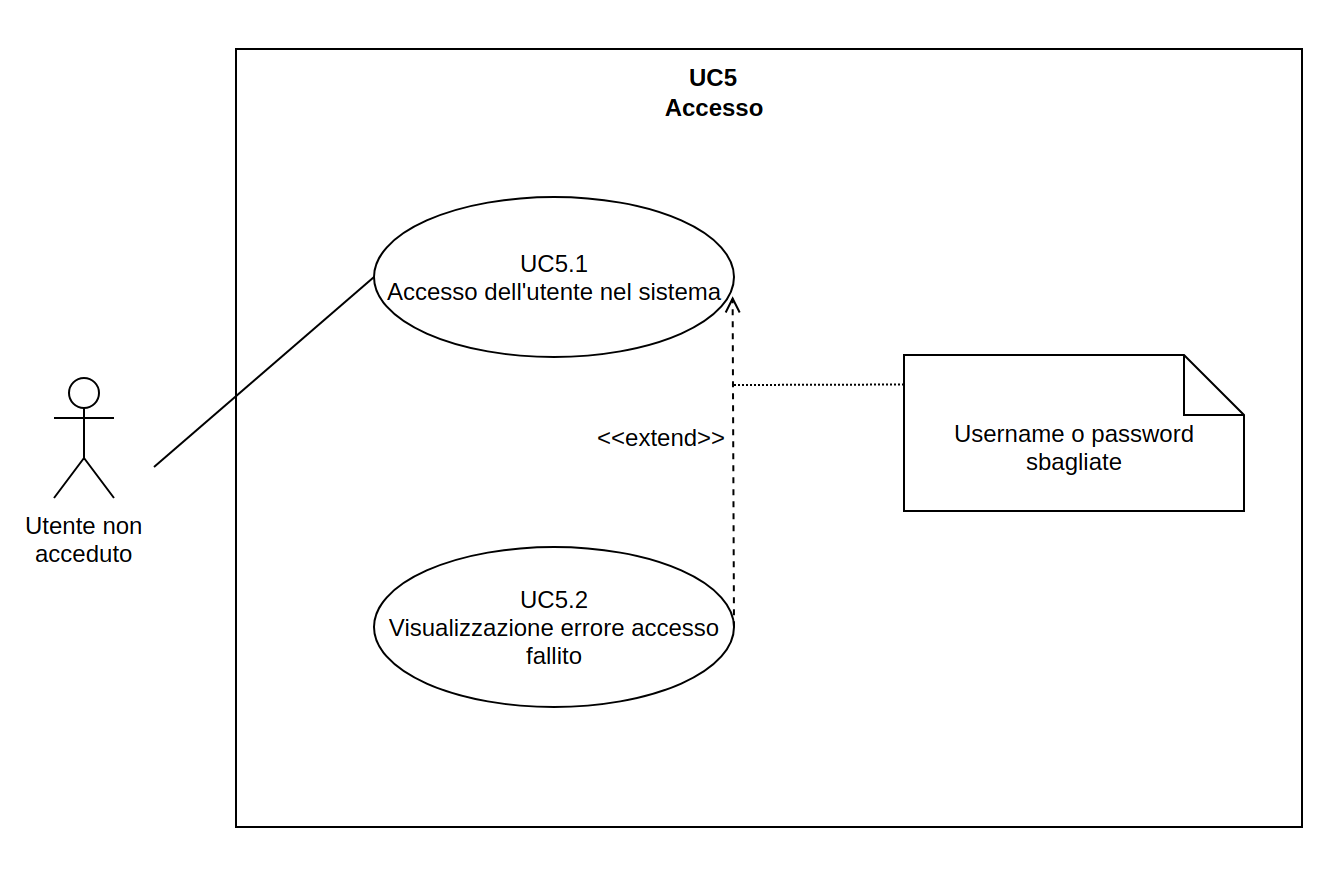
\includegraphics[width=\columnwidth]{img/UC5.png}\\
				\caption{UC\theuccount.1.1-GP - Inserimento nome utente}
			\end{figure}
			\begin{itemize}
				\item \textbf{Codice}: UC\theuccount.1.1-GP.
				\item \textbf{Titolo}: inserimento nome utente.
				\item \textbf{Attori primari}: utente acceduto.
				\item \textbf{Descrizione}: l'utente inserisce il nominativo dell'utente appena aggiunto.
				\item \textbf{Precondizione}: un nuovo utente deve essere aggiunto nel sistema.
				\item \textbf{Postcondizione}: il nome è stato aggiunto.
				\item \textbf{Scenario Principale}:
				\begin{enumerate}
					\item Utente acceduto procede all'aggiunta del nominativo del nuovo utente.
				\end{enumerate}
			\end{itemize}

			\subparagraph{UC\theuccount.1.2-GP - Inserimento cognome utente}
				\begin{figure}[H]
					\centering
					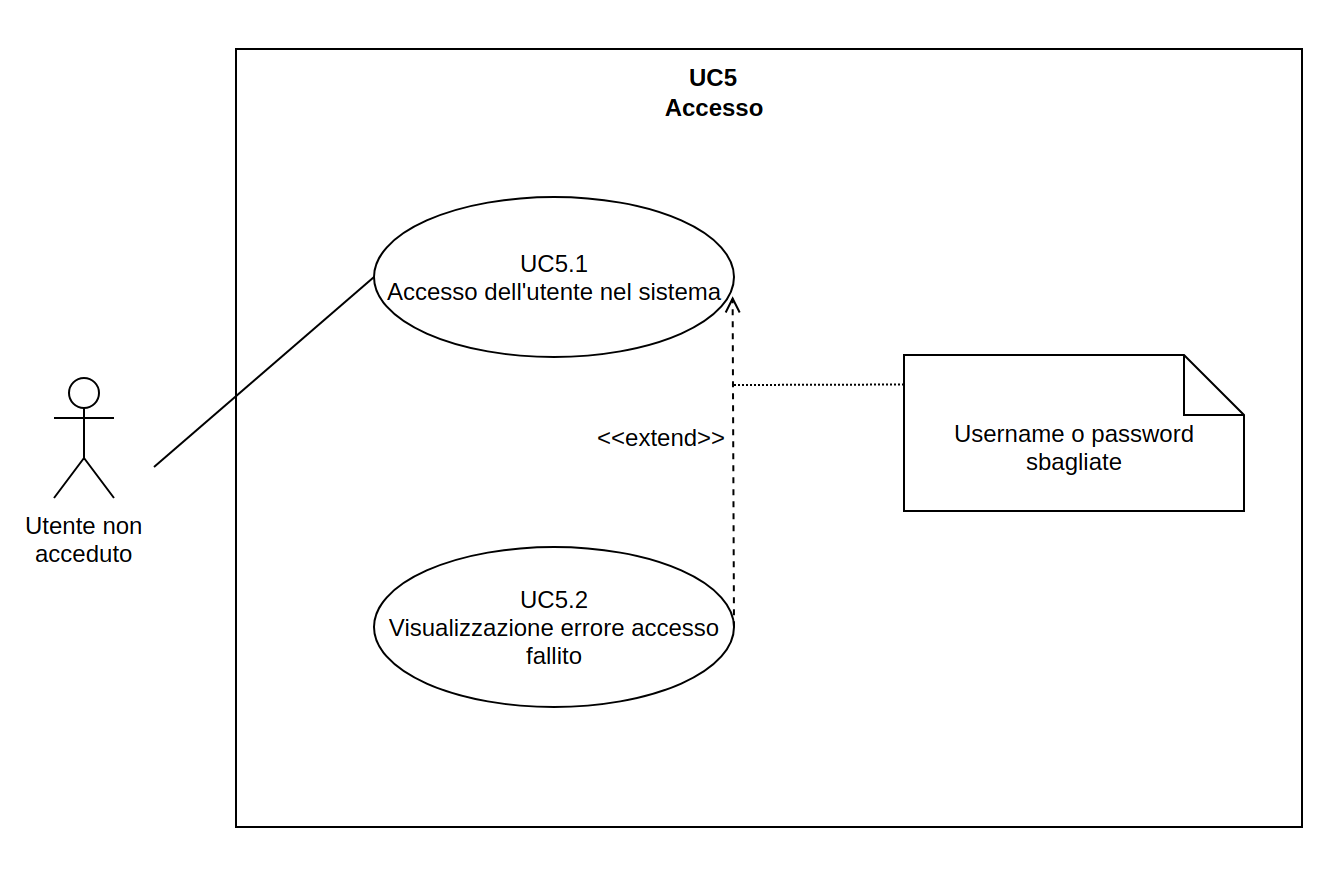
\includegraphics[width=\columnwidth]{img/UC5.png}\\
					\caption{UC\theuccount.1.2-GP - Inserimento cognome utente}
				\end{figure}
				\begin{itemize}
					\item \textbf{Codice}: UC\theuccount.1.2-GP.
					\item \textbf{Titolo}: inserimento cognome utente.
					\item \textbf{Attori primari}: utente acceduto.
					\item \textbf{Descrizione}: l'utente inserisce il cognome dell'utente appena aggiunto.
					\item \textbf{Precondizione}: un nuovo utente deve essere aggiunto nel sistema.
					\item \textbf{Postcondizione}: il cognome è stato aggiunto.
					\item \textbf{Scenario Principale}:
					\begin{enumerate}
						\item Utente acceduto procede all'aggiunta del cognome del nuovo utente.
					\end{enumerate}
				\end{itemize}

				\subparagraph{UC\theuccount.1.3-GP - Inserimento contatto Email}
					\begin{figure}[H]
						\centering
						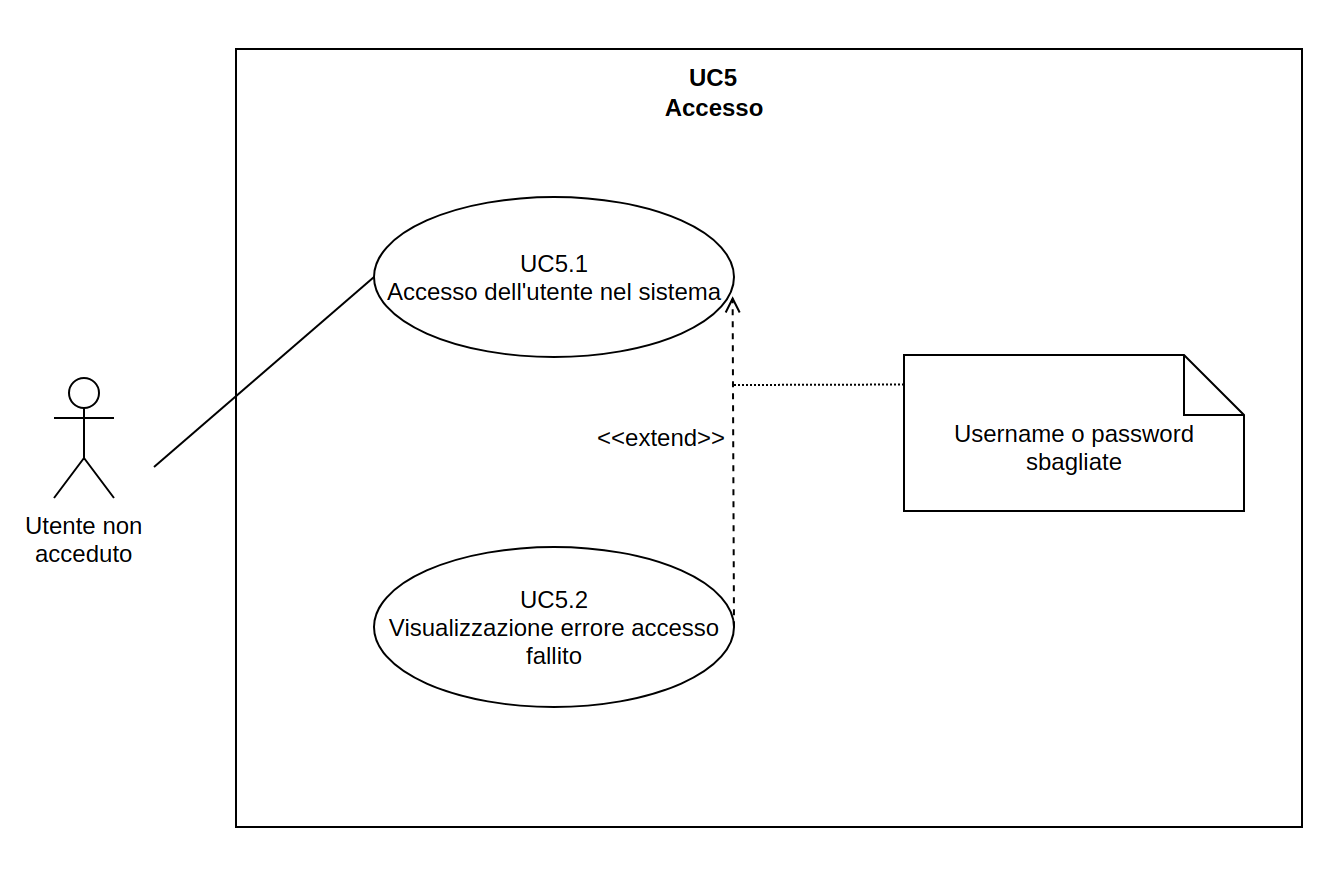
\includegraphics[width=\columnwidth]{img/UC5.png}\\
						\caption{UC\theuccount.1.3-GP - Inserimento contatto Email}
					\end{figure}
					\begin{itemize}
						\item \textbf{Codice}: UC\theuccount.1.3-GP.
						\item \textbf{Titolo}: inserimento contatto Email.
						\item \textbf{Attori primari}: utente acceduto.
						\item \textbf{Descrizione}: l'utente inserisce il contatto Email dell'utente appena aggiunto.
						\item \textbf{Precondizione}: un nuovo utente deve essere aggiunto nel sistema.
						\item \textbf{Postcondizione}: il contatto Email è stato aggiunto.
						\item \textbf{Scenario Principale}:
						\begin{enumerate}
							\item Utente acceduto procede all'aggiunta del contatto Email del nuovo utente.
						\end{enumerate}
				\end{itemize}

				\subparagraph{UC\theuccount.1.4-GP - Inserimento contatto Telegram}
					\begin{figure}[H]
						\centering
						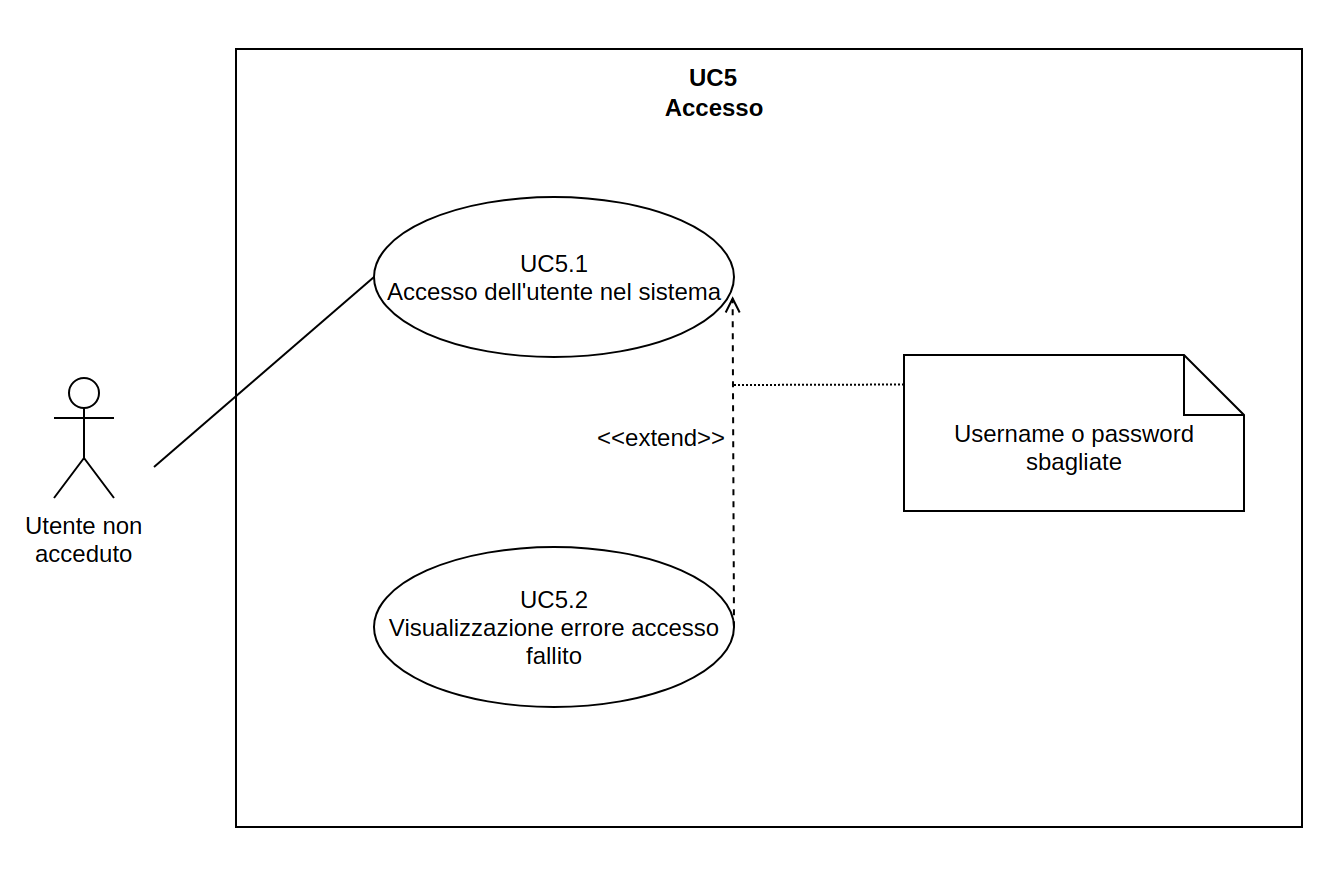
\includegraphics[width=\columnwidth]{img/UC5.png}\\
						\caption{UC\theuccount.1.4-GP - Inserimento contatto Telegram}
					\end{figure}
					\begin{itemize}
						\item \textbf{Codice}: UC\theuccount.1.4-GP.
						\item \textbf{Titolo}: inserimento contatto Telegram.
						\item \textbf{Attori primari}: utente acceduto.
						\item \textbf{Descrizione}: l'utente inserisce il contatto Telegram dell'utente appena aggiunto.
						\item \textbf{Precondizione}: un nuovo utente deve essere aggiunto nel sistema.
						\item \textbf{Postcondizione}: il contatto Telegram è stato aggiunto.
						\item \textbf{Scenario Principale}:
						\begin{enumerate}
							\item Utente acceduto procede all'aggiunta del contatto Telegram del nuovo utente.
						\end{enumerate}
					\end{itemize}

			\paragraph{UC\theuccount.2-GP - Errore utente già presente nel sistema}
				\begin{figure}[H]
					\centering
					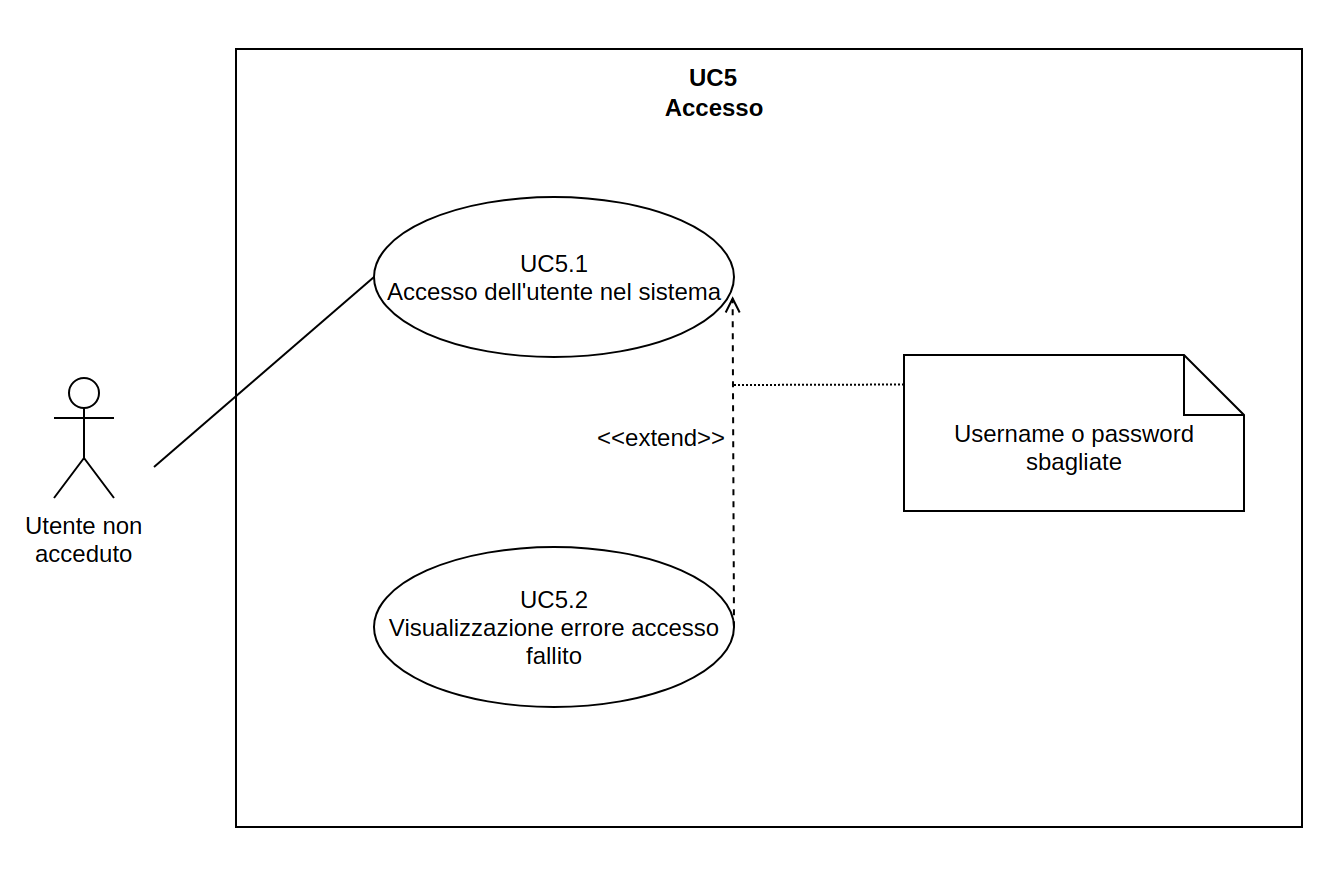
\includegraphics[width=\columnwidth]{img/UC5.png}\\
					\caption{UC\theuccount.2-GP - Errore utente già presente nel sistema}
				\end{figure}
				\begin{itemize}
					\item \textbf{Codice}: UC\theuccount.2-GP.
					\item \textbf{Titolo}: errore utente già presente nel sistema.
					\item \textbf{Attori primari}: utente acceduto.
					\item \textbf{Descrizione}: l’utente viene avvisato che i contatti Telegram o email immessi non sono univoci.
					\item \textbf{Precondizione}: un nuovo utente deve essere aggiunto nel sistema.
					\item \textbf{Postcondizione}: il sistema comunica all’utilizzatore l’errore e l'utente non viene inserito.
					\item \textbf{Scenario Principale}:
					\begin{enumerate}
						\item Utente acceduto visualizza il messaggio d'errore.
					\end{enumerate}
				\end{itemize}